% \begin{document}
\chapter{Riduzioni}

Le dimostrazioni dei teoremi del capitolo precedente avevano tutte un approccio simile: supponiamo per assurdo che un certo linguaggio sia decidibile, costruiamo una macchina ausiliaria sfruttando il decisore assunto esistere, e arriviamo a una contraddizione. Queste erano istanziazioni di un principio molto più generale: la \textbf{riduzione tra linguaggi}.

\dfn{Riduzione}{
  Siano $ A, B $ due linguaggi. La funzione $ f $ è una \textbf{riduzione} da $ A $ a $ B $ se per ogni stringa $ w $:
  \[
    w \in A \iff f(w) \in B
  \]
  e inoltre $ f $ è calcolabile. Quando esiste una riduzione da $ A $ a $ B $ scriviamo $ A \leq B $.
}

\nt{
  Intuitivamente, $ A \leq B $ significa che $ A $ non è più difficile di $ B $: saper risolvere $ B $ implica saper risolvere $ A $, applicando prima $ f $.
}

Per definire formalmente la calcolabilità di $ f $ è necessario introdurre un nuovo tipo di macchina.

\dfn{Trasduttore}{
  Un \textbf{trasduttore} è una Macchina di Turing che calcola funzioni, caratterizzata da tre nastri:
  \begin{enumerate}
    \item \textbf{Input} — sola lettura
    \item \textbf{Worktape} — lettura e scrittura
    \item \textbf{Output} — sola scrittura
  \end{enumerate}
  Un trasduttore $ M $ \textit{calcola} la funzione $ f $ se, per ogni stringa $ w $, quando $ M $ esegue su $ w $ e si arresta, lascia $ f(w) $ scritto sul nastro di output.
}

\nt{
  Distinguiamo trasduttori (calcolatori di funzioni) dalle MdT classiche (decisori). Una \textbf{funzione calcolabile} è una funzione per cui esiste un trasduttore che la calcola e che si arresta sempre in tempo finito su ogni input.
}

\section{Teorema sulle riduzioni}

\thm{}{
  Siano $ A, B $ due linguaggi tali che $ A \leq B $. Allora:
  \begin{enumerate}
    \item Se $ A \notin R \Rightarrow B \notin R $
    \item Se $ A \notin RE \Rightarrow B \notin RE $
  \end{enumerate}
}
\pf{Dimostrazione}{
  \textbf{Caso 1.} Supponiamo per assurdo che $ A \notin R $ ma $ B \in R $. Allora esiste $ M_B $ che decide $ B $. Costruiamo $ M_A $ su input $ w $:
  \begin{enumerate}
    \item Calcola $ f(w) $ tramite il trasduttore per $ f $
    \item Esegue $ M_B $ su $ f(w) $
    \item Risponde come $ M_B $
  \end{enumerate}
  Il trasduttore termina sempre per definizione di funzione calcolabile, e $ M_B $ termina sempre perché decide $ B $. La risposta è corretta poiché $ w \in A \iff f(w) \in B $. Quindi $ M_A $ decide $ A \Rightarrow A \in R $. Contraddizione.

  \textbf{Caso 2.} Supponiamo per assurdo che $ A \notin RE $ ma $ B \in RE $. Allora esiste $ M_B $ che accetta $ B $. Costruiamo $ M_A $ con la stessa pipeline di prima: calcola $ f(w) $ e poi esegue $ M_B $ su $ f(w) $. Allora:
  \begin{itemize}
    \item $ w \in A \Rightarrow f(w) \in B \Rightarrow M_B $ accetta $ \Rightarrow M_A $ accetta
    \item $ w \notin A \Rightarrow f(w) \notin B \Rightarrow M_B $ non accetta $ \Rightarrow M_A $ non accetta
  \end{itemize}
  Quindi $ M_A $ accetta $ A \Rightarrow A \in RE $. Contraddizione.
}

\cor{}{
  Siano $ A, B $ due linguaggi tali che $ A \leq B $. Allora:
  \[
    B \in R \Rightarrow A \in R \qquad\qquad B \in RE \Rightarrow A \in RE
  \]
}
\pf{Dimostrazione}{
  Segue direttamente per contronominale dal teorema precedente: $ (A \notin R \Rightarrow B \notin R) \equiv (B \in R \Rightarrow A \in R) $.
}

\nt{
  Nella pratica usiamo sempre il corollario in questa direzione: vogliamo dimostrare che $ B $ è difficile. Partiamo da un $ A $ noto essere indecidibile, mostriamo $ A \leq B $, e concludiamo che $ B $ non può essere decidibile — altrimenti lo sarebbe anche $ A $. TODO: ma allora non sarebbe il verso del teorema??
}

\section{Esempio: $ \mathcal{L}_{ne} $}

\dfn{$ \mathcal{L}_{ne} $}{
  \[
    \mathcal{L}_{ne} = \{M_i \mid \mathcal{L}(M_i) \neq \emptyset\}
  \]
  L'insieme delle MdT che accettano almeno una stringa.
}

\thm{}{
  
  $ \mathcal{L}_{ne} \in RE $
}
\pf{Dimostrazione}{
  Costruiamo la macchina $ M_{ne} $ che accetta $ \mathcal{L}_{ne} $. Data $ M_i $ in input, $ M_{ne} $ non sa a priori quale stringa $ M_i $ potrebbe accettare, quindi la \textbf{indovina} non deterministicamente (design pattern \textit{guess \& check}):
  \begin{enumerate}
    \item Indovina non deterministicamente una stringa $ w $
    \item Simula $ M_i $ su $ w $ tramite $ M_u $
    \item Se $ M_i $ accetta $ w $, risponde sì
  \end{enumerate}
  Se $ \mathcal{L}(M_i) \neq \emptyset $, esiste almeno una stringa $ w^* $ accettata da $ M_i $: un ramo non deterministico la indovinerà e risponderà sì in tempo finito. Non diamo garanzie sul no, ma per $ RE $ non è richiesto.
}

\thm{}{
  $ \mathcal{L}_{ne} \notin R $
}
\pf{Dimostrazione}{
  Mostriamo la riduzione $ \mathcal{L}_u \leq \mathcal{L}_{ne} $. Dobbiamo costruire una funzione $ f $ calcolabile tale che:
  \[
    (M, w) \in \mathcal{L}_u \iff f(M, w) \in \mathcal{L}_{ne}
  \]
  La funzione $ f $, data la coppia $ (M, w) $, costruisce una nuova macchina $ M' $ definita come segue: $ M' $ \textbf{ignora il proprio input} $ x $, scrive $ w $ sul nastro, e simula $ M $ su $ w $.

  Verifichiamo la correttezza di $ f $ in entrambe le direzioni:

  $ (\Rightarrow) $ Supponiamo $ (M, w) \in \mathcal{L}_u $, ovvero $ M \models w $. Allora $ M' $, su qualsiasi input $ x $, ignora $ x $, simula $ M $ su $ w $, e accetta — poiché $ M $ accetta $ w $. Quindi $ \mathcal{L}(M') = \Sigma^* \neq \emptyset $, da cui $ M' \in \mathcal{L}_{ne} $.

  $ (\Leftarrow) $ Supponiamo $ (M, w) \notin \mathcal{L}_u $, ovvero $ M \not\models w $. Allora $ M' $, su qualsiasi input $ x $, simula $ M $ su $ w $ e non accetta mai. Quindi $ \mathcal{L}(M') = \emptyset $, da cui $ M' \notin \mathcal{L}_{ne} $.

  La riduzione è corretta. Poiché $ \mathcal{L}_u \notin R $ e $ \mathcal{L}_u \leq \mathcal{L}_{ne} $, per il teorema sulle riduzioni segue $ \mathcal{L}_{ne} \notin R $.
}

\section{Corrispondenza di Post}
Andiamo a definire un problema che inizialmente sembra semplice, ma che usando le riduzioni puo' essere dimostrato che non appartiene a R: il \textbf{problema di corrispondenza di Post} (PCP).

\subsection{Definizione}

E' un problema di decisione:

\begin{itemize}
\item \textbf{Input}: lista di coppie di stringhe $ w \in \Sigma^* $ $ R, S  $ tale che $ |R| = |S| $
  \begin{center} 
  \begin{tabular}{c|c}
    $R(r_i)$ & $S(s_i)$ \\ \hline
    1 & 1 1 1 \\
    1 0 1 1 1 & 1 0 \\
    1 0 & 0 \\
  \end{tabular}
  \end{center}
\item \textbf{Output}: se esiste una sequenza di indici $ i_1, ..., i_u $ (con $ u > 0 $ per non essere banale) tale che
  \[
  r_{i_1} \cdot ... \cdot r_{i_u} = s_{i_1} \cdot ... \cdot s_{i_u}
  \]
  allora l'input e' accettato.
\end{itemize}

\ex{}{
  Per la costruzione di sopra, l'input $ R,S  $ e' accettato, dato che la sequenza
  \[
  2,1,1,3
  \]
  genera le stringhe
  \[
  r \to 101111110
  \]
  e 
  \[
  s \to 101111110
  \]
  che sono uguali.
}

\subsection{Appartenenza a RE}
Per dimostrare che PCP $ \in RE $, ci basta costruire una macchina (anche non deterministica) che riconosca il linguaggio associato al problema.\\

La soluzione e' abbastanza semplice: basta costruire una macchina non-deterministica che "indovina" (guess) la sequenza e che ne controlli (check) la validita'.

\subsection{Non-appartenenza a R}
Dobbiamo ora vedere se PCP appartiene o meno a $ R $, che coincide col trovare una macchina in grado di decidere il linguaggio del problema.\\

Intuitivamente si puo' vedere come, dato che le sequenze possibili sono infinite, il problema possa divergere. Ma vediamo come dimostrarlo:
\begin{itemize}
\item Riduciamo il linugaggio $ \mathcal{L}_u$ a un linguaggio intermedio $ MPCP $. Dato che il linguaggio universale e' indecidibile, lo e' anche $ MPCP $.
\item Facciamo una seconda riduzione da $ MPCP $ a $ PCP $, e per lo stesso motivo questo significa che $ PCP \not\in R $. 
\end{itemize}

Quindi
\[
  \mathcal{L}_u \leq MPCP \leq PCP
\]
Il linguaggio $ MPCP $ e' molto simile a $ PCP $, ma le sequenze accettate devono iniziare tutte con il primo indice.

\subsubsection{Riduzione a MPCP}

Guardiamo la prima riduzione $ \mathcal{L}_u \leq MPCP$ e facciamoci le solite domande

\begin{enumerate}
\item Qual'e' il problema di partenza? E quello di arrivo?
\item Quali sono gli input dei due problemi?
\item Quali sono le istanze si dei due problemi? E le istanze no?
\item Come facciamo a trasformare istanze si del problema di partenza in istanze si del problema di arrivo e stessa cosa per le istanze no?
\end{enumerate}

Sappiamo che l'input al problema di partenza sono le coppie macchina/stringa $ (M,w) $ e le sue istanze si' sono le coppie dove $ M $ accetta $ w $, mentre le no sono quelle dove $ M $ non accetta $ w $.\\

Dobbiamo trovare ora una funzione calcolabile $ f $ che prende gli input di $ \mathcal{L}_u $ e li trasforma in input di $ MPCP $ in modo che: se $ (M,w) $ e' un'istanza si, allora $ f((M,w)) $ e' un'istanza si di $ MPCP $; e se e' un'istanza no, allora $ f((M,w)) $ e' un'istanza no di $ MPCP $.

\nt{
  ATTENZIONE: puo' sembrare possibile definire $ f $ come la funzione che "simula" $ w $ su $ M $ e se accetta allora crea un'istanza si banale per MPCP, altrimenti ne crea una no banale. Ma questo non e' possibile dato che $ \mathcal{L}_u \not\in R$ quindi $ f $ puo' divergere, rendendola non-calcolabile. 
}

Ricordiamoci che una computazione di una MdT puo' essere scritta come una sequenza di configurazioni.

\ex{}{ \label{es:comp}
  \begin{center}
    
\includegraphics[width=0.5\textwidth]{img/2026-03-16-19-11-14.png}
  \end{center}
  Dato in input $ w = 01 $, otteniamo la seguente computazione
  \[
  q_1 01 \vdash 1q_2 1 \vdash 10q_1 \vdash 1q_2 01 \vdash q_3 101
  \]
  dove l'ultima e' una configurazione accettante.
}
L'idea e' quella di guardare la funzione di transizione della macchina $ M $ e la stringa in input $ w $ per poi impostare le stringhe in $ R $ e in $ S $ in modo tale che se esiste una computazione di $ M $ per $ w $, allora esiste una sequenza per cui $ r = s  $, che e' la stringa che rappresenta la computazione. Al contrario, se non esiste una computazione allora non esistera' nessuna sequenza per cui $ r = s  $.\\

Proviamo a guardare un esempio di come possiamo costruire una tale funzione sulla macchina \ref{es:comp}:

\begin{center}
  \begin{tabular}{c|c}
    $ R $ & $ S $ \\ \hline
    $ \# $ & $ \# q_1 01 \# $ \\
    $ q_1 0 $ & $ 1q_2 $\\
    $ 1 $ & $ 1 $\\
    $ \# $ & $ \# $\\
    $ q_2 1 $ & $ 0 q_1 $\\
    $ 0q_1\# $ & $ q_2 01 $\\
    $ 1q_2 0 $ & $ q_3 1 0 $\\
    $ q_3 1 $ & $ q_3 $\\
    $ q_3 0 $ & $ q_3 $\\
    $ q_3 \#\# $ & $ \# $
  \end{tabular}
\end{center}

Per come abbiamo costruito $ R $ e $ S  $, vediamo che c'e' una soluzione al problema MPCP che e' la seguente:

\[
r = s = \# q_1 01 \# 1q_2 1 \# 10q_1 \# 1q_2 01 \# q_3 101 \# q_3 01 \# q_3 1 \# q_3 \# \# 
\]
che e' proprio la computazione della stringa $ w $ con delle parti finali aggiuntive.\\

Abbiamo infatti costruito $ R $ in modo da essere un "passo" piu' indietro rispetto a $ S  $ nella computazione, ovvero se su $ r_i $ leggo una configurazione allora su $ s_i $ avro' il suo legal successor. Quando $ s  $ raggiunge lo stato accettante (quindi $ w $ e' accettata), $ r $ fa un "passo" in piu' per pareggiare le due stringhe.\\

In questo modo, se esiste una computazione per $ w = 01 $ le due stringhe possono ricongiungersi; ma se $ s  $ non arriva mai ad una configurazione accettante, allora $ r $ sara' sempre un passo indietro.\\

Formalizziamo questa idea definendo una costruzione della coppia $ (R,S) $ a partire da $ (M,w) $, distinguendo 5 parti:
\begin{center}
  \begin{tabular}{ll|ll}
    &$ R $ & $ S $ & \\ \hline
    &$ \# $ & $ \# q_0 w_1...w_n $ & \\ \hline
    $ \forall x \in \Gamma $&$ x $ & $ x $ & \\
    &$ \# $ & $ \# $ &\\ \hline
    $ \forall q \in Q \setminus F, $&$ qx $ & $ yp $ & $ \delta (q,x) = (p, y, \to) $\\
    $ \forall x,y,z \in \Gamma $&$ zqx $ & $ pzy $ & $ \delta (q,x) = (p, y, \gets) $\\
    &$ q\# $ & $ yp\# $ & $ \delta (q,\cancel{b}) = (p, y, \to) $\\
    &$ zq\# $ & $ pzy\# $ & $ \delta (q,\cancel{b}) = (p, y, \gets) $\\ \hline
    $ \forall q \in F, $&$ xqy $&$ q  $&\\
    $ \forall x,y,z \in \Gamma $&$ xq $&$ q  $&\\
    &$ qy $&$ q  $&\\ \hline
    $ \forall q \in F $&$ q\#\# $&$ \#  $&
  \end{tabular}
\end{center}

Controlliamo che $ f $ sia effettivamente la trasformazione che stavamo cercando:
\begin{itemize}
\item E' una funzione calcolabile?\\
  \textbf{Si'}, dato che che non ci serve sapere se $ M $ accetta $ w $, ma costruisce solo un numero finito di coppie di stringhe guardando la funzione di transizione di $ M $.
\item Se $ (M,w) \in \mathcal{L}_u $, e' vero che $ f(M,w) $ e' un'istanza si' di $ MPCP $?\\
  \textbf{Si'}, dato che per ogni $ w $ accettata da $ M $ esiste una sequenza che simula l'esecuzione di $ M $ su $ w $.
\item Se $ (M,w) \not\in \mathcal{L}_u $, e' vero che $ f(M,w) $ e' un'istanza no di $ MPCP $?\\
  \textbf{Si'}, dato che se $ f(M,w) = (R,S) $ e' un'istanza si di $ MPCP $, allora esiste una sequenza che inizia con la configurazione iniziale di $ M $ su $ w $ e finisce in una configurazione accettante rispettando la funzione di transizione di $ M $, quindi $ M $ accetta $ w $ quindi $ (M,w) \in \mathcal{L}_u $. Dato che abbiamo dimostrato il contra-positivo, abbiamo dimostrato la premessa iniziale.
\end{itemize}

\subsubsection{Riduzione a PCP}
Ci basta ora trovare la seconda riduzione $ MPCP \leq PCP $.

Dopo aver risposto alle solite domande, non rimane che costruire la funzione $ f $:
\begin{center}
  \begin{tabular}{c|c}
    $ R $ & $ S  $\\ \hline
    1 & 111\\
    10111 & 10\\
    10 & 0
  \end{tabular} $ \longrightarrow $
  \begin{tabular}{c|c}
    T & U\\ \hline
    *1* & *1*1*1\\ \hline
    1* & *1*1*1\\
    1*0*1*1*1* & *1*0\\
    1*0* & *0\\ \hline
    \$ & *\$
\end{tabular}
\end{center}

Stiamo aggiungendo un carattere speciale a sinistra di ogni carattere delle stringhe in $ R $ e a destra di ogni carattere delle stringhe in $ S  $. In questo modo e' impossibile chesia un'istanza si di $ PCP $ dato che $ t $ iniziera' sempre con il carattere speciale e $ u $ no.\\

Aggiungiamo quindi una coppia $ t_0 = *t_1 , u_0 = u_1 $ in modo che, se esiste una sequenza che risolva il problema, allora il primo indice della sequenza $ i_1 $ e' per forza 0.\\

Dobbiamo inoltre aggiungere un carattere speciale alla fine di $ u $, quindi aggiungiamo una coppia $ t_{k+1} = \$, u_{k+1} = *\$ $ in modo che, se esiste una sequenza che risolva il problema, allora l'ultimo indice di tale sequenza e' per forza $ k + 1 $.\\

Controlliamo che $ f $ sia effettivamente la trasformazione che stavamo cercando:
\begin{itemize}
\item E' una funzione calcolabile?\\
  \textbf{Si'}, non fa nulla di crazy.
\item Se $ (R,S) $ e' un'istanza si' di $ MPCP $, e' vero che $ f(R,S) = (T,U) $ e' un'istanza si' di $ PCP $?\\
  \textbf{Si'}, dato che sia $ r_1r_{i_2}...r_{i_n} = s_1s_{i_2}...s_{i_n} $ una sequenza di $ (R,S) $, allora la sequenza $ t_0t_{i_2}...t_{i_n}t_{k+1} = u_0u_{i_2}...u_{i_n} u_{k+1} $ e' un'istanza si' di $ PCP $.
\item Se $ (R,S)$ e' un'istanza no di $ MPCP $, e' vero che $ f(R,S) $ e' un'istanza no di $ MPCP $?\\
  \textbf{Si'}, dato che se $ f(R,S) = (T,U) $ e' un'istanza si di $ PCP $, allora per le proprieta' di $ f $ indicate prima, $ t $ e $ u $ devono iniziare con $ t_0/u_0 $ e finire con $ t_{k+1}/u_{k+1} $:
    \[
    t_0t_{i_2}...t_{i_n}t_{k+1} = u_0u_{i_2}...u_{i_n}u_{k+1}
    \]
    Tralasciando l'ultimo indice e considerando $ i_1 = 1 $, vediamo come
    \[
    r_1r_{i_2}...r_{i_n} = s_1s_{i_2}...s_{i_n}
    \]
    e' una soluzione al problema $ MPCP $, quindi $ (R,S) $ e' un'istanza si. Dato che abbiamo dimostrato il contra-positivo, abbiamo dimostrato la premessa iniziale.
\end{itemize}

\section{Il Problema del Tassellamento}
 
\subsection{Definizione informale}
 
Si consideri un piano quadrettato infinito (il primo quadrante di $\mathbb{N}\times\mathbb{N}$).
Abbiamo un numero finito di \emph{tipi di piastrelle}, ciascuna con i quattro lati
colorati. Una piastrella speciale $S$ (o $d_0$) deve essere posizionata nell'origine
$(0,0)$.
 
Le piastrelle possono essere affiancate \emph{solo ``a domino''}: i bordi a contatto
devono avere lo stesso colore. \textbf{Non è consentita la rotazione.}
 
\begin{center}
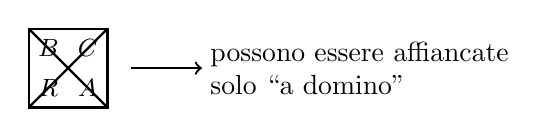
\begin{tikzpicture}
  % Tile with labels B, C (top-left), A (right), R (bottom-right)
  \draw[thick] (0,0) rectangle (1,1);
  \draw[thick] (0,0) -- (1,1);
  \draw[thick] (1,0) -- (0,1);
  \node at (0.25,0.75) {\small $B$};
  \node at (0.75,0.75) {\small $C$};
  \node at (0.75,0.25) {\small $A$};
  \node at (0.25,0.25) {\small $R$};
  \draw[->, thick] (1.3, 0.5) -- (2.2, 0.5);
  \node[align=left] at (4.2, 0.5) {possono essere affiancate\\solo ``a domino''};
\end{tikzpicture}
\end{center}
 
\medskip
\noindent
\textbf{Domanda:} È possibile ricoprire l'intero primo quadrante affiancando le
piastrelle (senza ruotarle)?
 
\subsection{Formalizzazione}
 
\dfn{Sistema di tassellamento}{
Un \emph{sistema di tassellamento} è una quadrupla
\[
  T = (D,\, d_0,\, H,\, V)
\]
dove:
\begin{itemize}
  \item $D$ è l'insieme finito dei \emph{tipi di piastrelle};
  \item $d_0 \in D$ è la \emph{piastrella speciale} (l'unica che può stare in
        posizione $(0,0)$);
  \item $H \subseteq D \times D$ sono le \emph{regole di affiancamento orizzontale}:
        $(a,b)\in H$ significa che $a$ può stare immediatamente a sinistra di $b$;
  \item $V \subseteq D \times D$ sono le \emph{regole di affiancamento verticale}:
        $(a,b)\in V$ significa che $a$ può stare immediatamente sotto $b$.
\end{itemize}
}
 
\dfn{Tassellamento valido}{
  Una funzione $f : \mathbb{N} \times \mathbb{N} \to D$ è un \emph{tassellamento valido} per $T$ se:
\begin{align}
  f(0,0) &= d_0, \label{eq:initial}\\
  \bigl(f(m,n),\, f(m+1,n)\bigr) &\in H \quad \forall m,n \in \mathbb{N}, \label{eq:horiz}\\
  \bigl(f(m,n),\, f(m,n+1)\bigr) &\in V \quad \forall m,n \in \mathbb{N}. \label{eq:vert}
\end{align}
}
 
Il \textbf{Problema del Tassellamento} (Tiling) è:
\[
  \text{Tiling} = \{\, T = (D, d_0, H, V) \mid \exists f : \mathbb{N}\times\mathbb{N} \to D
  \text{ tassellamento valido per } T \,\}.
\]
  
\subsection{Indecidibilita' del Tassellamento}
 
Vogliamo dimostrare che Tiling è indecidibile. Per farlo mostriamo che
\[
  \overline{\mathrm{HALT}_\varepsilon} \;\leq\; \text{Tiling},
\]
dove $\mathrm{HALT}_\varepsilon = \{\,M \mid M \text{ si ferma su } \varepsilon\,\}$ e
$\overline{\mathrm{HALT}_\varepsilon}$ è il suo complementare (le macchine che \emph{non} si fermano su~$\varepsilon$).
 
Poiché $\overline{\mathrm{HALT}_\varepsilon} \notin \mathrm{RE}$, dalla riduzione segue che
Tiling $\notin \mathrm{RE}$, in particolare è indecidibile.
  
Definiamo una funzione calcolabile
\[
  g : \text{Macchine di Turing} \;\longrightarrow\; \text{Sistemi di tassellamento},
  \quad M \;\longmapsto\; T = g(M),
\]
tale che:
\begin{itemize}
  \item Se $M$ \textbf{non si ferma} su $\varepsilon$ (cioè $M \notin \mathrm{HALT}_\varepsilon$),
        allora $\exists f$ per $T$, ossia $T \in \text{Tiling}$.
      \item Se $M$ \textbf{si ferma} su $\varepsilon$ (cioè $M \in \mathrm{HALT}_\varepsilon$),
        allora $\nexists f$ per $T$, ossia $T \notin \text{Tiling}$.
\end{itemize}
  
Se $M$ diverge su $\varepsilon$, la computazione è infinita:
\[
  c_1 \vdash c_2 \vdash c_3 \vdash \cdots
\]
Ogni configurazione $c_i$ viene ``tradotta'' in una riga del piano.
 
\begin{center}
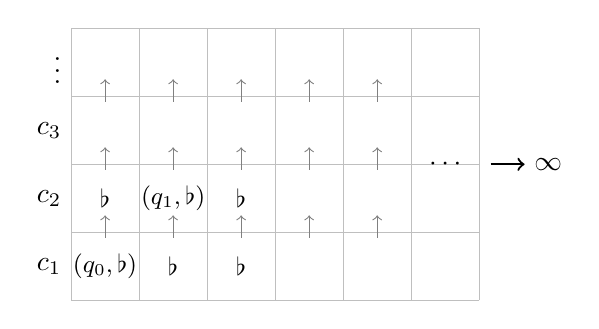
\begin{tikzpicture}[scale=0.72]
  % Grid
  \draw[step=1.2cm, gray!50, thin] (0,0) grid (7.2, 4.8);
  % Row labels
  \node[left] at (0, 0.6) {$c_1$};
  \node[left] at (0, 1.8) {$c_2$};
  \node[left] at (0, 3.0) {$c_3$};
  \node[left] at (0, 4.2) {$\vdots$};
  % Sample cell labels (first row, cells 0..2)
  \node[font=\small] at (0.6, 0.6) {$(q_0,\flat)$};
  \node[font=\small] at (1.8, 0.6) {$\flat$};
  \node[font=\small] at (3.0, 0.6) {$\flat$};
  % second row
  \node[font=\small] at (0.6, 1.8) {$\flat$};
  \node[font=\small] at (1.8, 1.8) {$(q_1,\flat)$};
  \node[font=\small] at (3.0, 1.8) {$\flat$};
  % arrows
  \foreach \x in {0.6, 1.8, 3.0, 4.2, 5.4} {
    \draw[->, gray] (\x, 1.1) -- (\x, 1.5);
    \draw[->, gray] (\x, 2.3) -- (\x, 2.7);
    \draw[->, gray] (\x, 3.5) -- (\x, 3.9);
  }
  \node at (6.6, 2.4) {$\cdots$};
  \draw[->, thick] (7.4, 2.4) -- (8.0, 2.4);
  \node[right] at (8.0, 2.4) {$\infty$};
\end{tikzpicture}
\end{center}
 
\noindent\textbf{Intuizione:} se la sequenza $c_1, c_2, \ldots$ è infinita, allora
è possibile piastrellare tutto il piano.
 
 
\paragraph{Colori (lati delle piastrelle).}
I colori codificano coppie (stato, simbolo) oppure semplici simboli del nastro:
\[
  \underbrace{q_0\flat,\quad \flat,\quad q_1\flat,\quad \ldots}_{\text{coppie (stato, simbolo)}},
  \qquad
  \underbrace{\vec{q}_1,\quad \vec{q}_0,\quad \ldots}_{\text{stati con direzione}}
\]
 
\paragraph{Tipi di piastrelle.}
 
Per codificare la computazione di $M$ costruiamo $D$, $H$ e $V$ come segue. Ogni
piastrella è un quadratino con quattro lati colorati (basso, alto, sinistra, destra).
Usiamo la notazione diagonale:
\[
  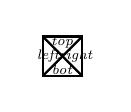
\begin{tikzpicture}[baseline=-0.5ex,scale=0.5]
    \draw[thick] (0,0) rectangle (1,1);
    \draw[thick] (0,0)--(1,1); \draw[thick](1,0)--(0,1);
    \node[font=\tiny] at (0.5,0.15) {$\mathit{bot}$};
    \node[font=\tiny] at (0.5,0.85) {$\mathit{top}$};
    \node[font=\tiny] at (0.15,0.5) {$\mathit{left}$};
    \node[font=\tiny] at (0.85,0.5) {$\mathit{right}$};
  \end{tikzpicture}
\]
 
\noindent
Costruiamo tre famiglie di piastrelle:
 
\begin{enumerate}[label=\textbf{\arabic*)}]
 
\item \textbf{Piastrelle di propagazione (per ogni $x \in \Gamma$).}\\
  Per ogni simbolo $x$ del nastro, una piastrella che porta il simbolo al livello
  superiore senza modificarlo:
  \begin{center}
  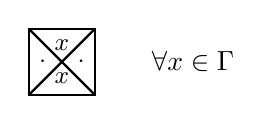
\begin{tikzpicture}[scale=0.7]
    \draw[thick] (0,0) rectangle (1.2,1.2);
    \draw[thick] (0,0)--(1.2,1.2); \draw[thick](1.2,0)--(0,1.2);
    \node[font=\small] at (0.6, 0.9) {$x$};
    \node[font=\small] at (0.6, 0.3) {$x$};
    \node[font=\small] at (0.25, 0.6) {$\cdot$};
    \node[font=\small] at (0.95, 0.6) {$\cdot$};
    \node[right=0.6cm] at (1.2,0.6) {$\forall x \in \Gamma$};
  \end{tikzpicture}
  \end{center}
  Questi permettono di portare i simboli al livello sopra.
 
\item \textbf{Piastrelle di transizione $\to$ (mossa a destra).}\\
  Per ogni transizione $\delta(q, x) = (p, y, \to)$ e per ogni $z \in \Gamma$,
  si generano due piastrelle adiacenti:
 
  \begin{center}
  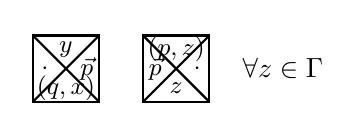
\begin{tikzpicture}[scale=0.7]
    % left tile: bottom=(q,x), top=y, right=arrow_p
    \draw[thick] (0,0) rectangle (1.2,1.2);
    \draw[thick] (0,0)--(1.2,1.2); \draw[thick](1.2,0)--(0,1.2);
    \node[font=\small] at (0.6,0.25) {$(q,x)$};
    \node[font=\small] at (0.6,0.95) {$y$};
    \node[font=\small] at (0.22,0.6) {$\cdot$};
    \node[font=\small] at (0.98,0.6) {$\vec{p}$};
    % right tile: bottom=z, top=(p,z), left=arrow_p
    \draw[thick] (2,0) rectangle (3.2,1.2);
    \draw[thick] (2,0)--(3.2,1.2); \draw[thick](3.2,0)--(2,1.2);
    \node[font=\small] at (2.6,0.25) {$z$};
    \node[font=\small] at (2.6,0.95) {$(p,z)$};
    \node[font=\small] at (2.22,0.6) {$\vec{p}$};
    \node[font=\small] at (2.98,0.6) {$\cdot$};
    \node[right=0.3cm] at (3.2,0.6) {$\forall z \in \Gamma$};
  \end{tikzpicture}
  \end{center}
 
\item \textbf{Piastrelle di transizione $\leftarrow$ (mossa a sinistra).}\\
  Per ogni transizione $\delta(q, x) = (p, y, \leftarrow)$ e per ogni $z \in \Gamma$:
 
  \begin{center}
  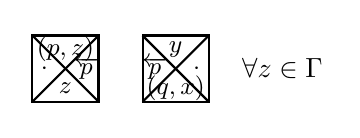
\begin{tikzpicture}[scale=0.7]
    % left tile: bottom=z, top=(p,z), right=arrow_p_left
    \draw[thick] (0,0) rectangle (1.2,1.2);
    \draw[thick] (0,0)--(1.2,1.2); \draw[thick](1.2,0)--(0,1.2);
    \node[font=\small] at (0.6,0.25) {$z$};
    \node[font=\small] at (0.6,0.95) {$(p,z)$};
    \node[font=\small] at (0.22,0.6) {$\cdot$};
    \node[font=\small] at (0.98,0.6) {$\overleftarrow{p}$};
    % right tile: bottom=(q,x), top=y, left=arrow_p_left
    \draw[thick] (2,0) rectangle (3.2,1.2);
    \draw[thick] (2,0)--(3.2,1.2); \draw[thick](3.2,0)--(2,1.2);
    \node[font=\small] at (2.6,0.25) {$(q,x)$};
    \node[font=\small] at (2.6,0.95) {$y$};
    \node[font=\small] at (2.22,0.6) {$\overleftarrow{p}$};
    \node[font=\small] at (2.98,0.6) {$\cdot$};
    \node[right=0.3cm] at (3.2,0.6) {$\forall z \in \Gamma$};
  \end{tikzpicture}
  \end{center}
 
\item \textbf{Piastrella iniziale $d_0$.}\\
  La piastrella speciale che forza la prima riga a contenere $c_1 = (q_0, \flat)$:
 
  \begin{center}
  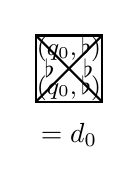
\begin{tikzpicture}[scale=0.7]
    \draw[thick] (0,0) rectangle (1.2,1.2);
    \draw[thick] (0,0)--(1.2,1.2); \draw[thick](1.2,0)--(0,1.2);
    \node[font=\small] at (0.6,0.25) {$(q_0,\flat)$};
    \node[font=\small] at (0.6,0.95) {$(q_0,\flat)$};
    \node[font=\small] at (0.25,0.6) {$\flat$};
    \node[font=\small] at (0.95,0.6) {$\flat$};
    \node[below=0.15cm] at (0.6,0) {$= d_0$};
  \end{tikzpicture}
  \end{center}
 
\end{enumerate}
 
\subsubsection{Correttezza della riduzione}
 
\mlenma{}{
La funzione $g$ è calcolabile.
}
\pf{Dimostrazione}{
$D$, $H$, $V$ si calcolano in modo effettivo a partire dalla descrizione di $M$:
basta enumerare le transizioni e generare le piastrelle corrispondenti.
}
 
\thm{}{
  $M \notin \mathrm{HALT}_\varepsilon \;\Longleftrightarrow\; g(M) \in \mathrm{Tiling}$.
}
\pf{Dimostrazione}{
\textbf{($\Rightarrow$)} Sia $M$ una macchina che \emph{non} si ferma su $\varepsilon$.
Allora la computazione è infinita: $c_1 \vdash c_2 \vdash \cdots$
 
Per definizione di $g(M) = T$, abbiamo la possibilità di estendere le righe
all'infinito: la riga $n$ del tassellamento codifica la configurazione $c_n$.
La funzione $f(m,n) = \text{(tipo della cella } m \text{ nella configurazione } c_n)$
è un tassellamento valido per $T$.
 
\textbf{($\Leftarrow$)} Sia $T = g(M)$ ammette un tassellamento $f$.
Per costruzione, la riga 0 è forzata a contenere le piastrelle speciali che
codificano $c_1$. Ogni riga deve essere la configurazione successiva, dunque $f$
codifica una computazione infinita $c_1 \vdash c_2 \vdash \cdots$, il che implica
  $M \notin \mathrm{HALT}_\varepsilon$.
 
  Per contrapposizione: $M \in \mathrm{HALT}_\varepsilon \Rightarrow g(M) \notin \mathrm{Tiling}$.
}
 
\cor{}{
Il Problema del Tassellamento è indecidibile.
}
 
\section{Teoria della Ricorsione: gerarchia RE/R/co-RE}

Abbiamo visto molti problemi di decisione per i quali e' sempre possibile accettare una stringa in tempo finito, ma se l'input e' un'istanza no allora non abbiamo la garanzia che la macchina termini. Questi linguaggi, che possono essere solo riconosciuti da MdT, appartengono a $ RE \setminus R $, ma cosa succede se guardiamo i loro complementari? Vediamo un esempio:
\begin{itemize}
  \item $L_u = \{(M,w) \mid M \text{ si ferma su } w\}$: è un problema in $\mathrm{RE}$,
        abbiamo una procedura per rispondere sì in tempo finito.
  \item $\overline{L_u}$: è un problema che deve arrivare all'infinito per dire sì,
    quindi $\overline{L_u} \notin \mathrm{RE}$. Ma e' possibile dire di no in tempo finito.
\end{itemize}
 
Tutti questi problemi ($ \overline{L_u}, L_d, \overline{HALT}, \overline{HALT_\varepsilon},... $) hanno il complementare in $\mathrm{RE}$, quindi possiamo dire no in tempo finito. Questa proprieta' ci permette di definire una terza classe di calcolabilita':
 
\dfn{Classe co-RE}{
  Chiamiamo \textit{co-RE} la classe di linguaggi il cui complemento appartiene a RE
  \[
  co-RE = \{L | \overline{L} \in RE\}
  \]
}
 
\subsection{Teoremi fondamentali}
 
\thm{}{\label{thm:rneqre}
  $\mathrm{R} \neq \mathrm{RE}$
}
\pf{Dimostrazione}{
  $\exists L \in \mathrm{RE}$ con $L \notin \mathrm{R}$: ad esempio $\mathrm{HALT}_\varepsilon \in \mathrm{RE} \setminus \mathrm{R}$.
}
 
\thm{}{\label{thm:corere}
  $\mathrm{coRE} \cap \mathrm{RE} = \mathrm{R}$
}
\pf{Dimostrazione}{
  \textbf{($\mathrm{coRE} \cap \mathrm{RE} \subseteq \mathrm{R}$):} Sia $L \in \mathrm{coRE} \cap \mathrm{RE}$.
  Se $L \in \mathrm{coRE}$, allora $\overline{L} \in \mathrm{RE}$.
  Ma se $L \in \mathrm{RE}$ e $\overline{L} \in \mathrm{RE}$, allora $L \in \mathrm{R}$
(si eseguono in parallelo i due semidecisori e si risponde quando uno dei due
si ferma).
 
  \textbf{($\mathrm{R} \subseteq \mathrm{coRE} \cap \mathrm{RE}$):} Sia $L \in \mathrm{R}$; allora esiste $H$ che
  decide $L$. Tale $H$ risponde sì ($\in \mathrm{RE}$) e risponde no ($\in \mathrm{coRE}$).
}
 
\thm{}{\label{thm:reneqcore}
  $\mathrm{RE} \neq \mathrm{coRE}$
}
\pf{Dimostrazione}{
  Per il Teorema~\ref{thm:corere}, $\mathrm{coRE} \cap \mathrm{RE} = \mathrm{R}$.
  Se fosse $\mathrm{RE} = \mathrm{coRE}$, allora $\mathrm{RE} = \mathrm{R}$, contraddicendo il Teorema~\ref{thm:rneqre}.
}

Date queste proprieta' possiamo costruire il seguente diagramma:
\begin{center}
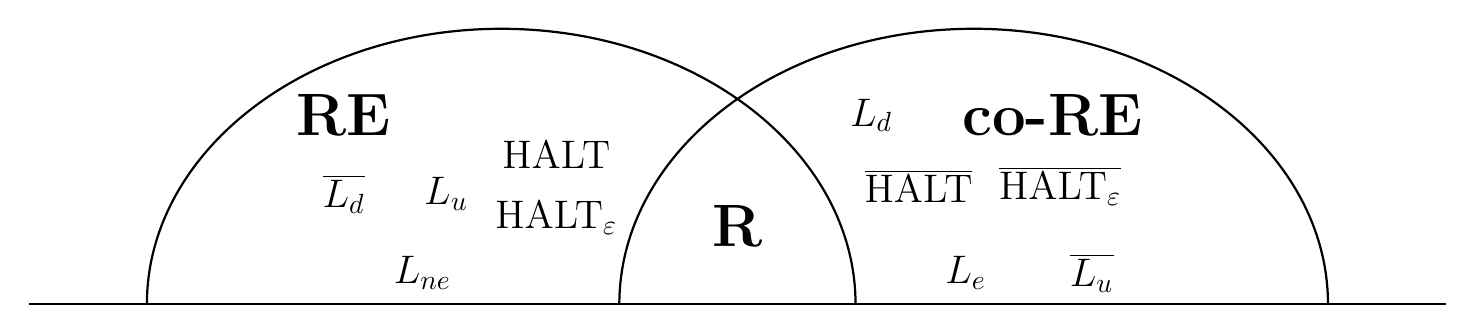
\begin{tikzpicture}[
    thick,
    font=\Large,
    draw=black,
    text=black
]

    % Horizontal base line
    \draw (-9, 0) -- (9, 0);

    % Left dome (representing RE)
    % Center is at (-1, 0), radius is 4.5 wide, 3.5 high
    \draw (-7.5, 0) arc (180:0:4.5cm and 3.5cm);

    % Right dome (representing coRE)
    % Center is at (1, 0), radius is 4.5 wide, 3.5 high
    \draw (-1.5, 0) arc (180:0:4.5cm and 3.5cm);

    % --- Center Intersection ---
    \node[scale=1.5] at (0, 1) {\textbf{R}};

    % --- Left Side (RE Region) ---
    \node[scale=1.5] at (-5, 2.4) {\textbf{RE}};
    \node at (-5, 1.4) {$\overline{L_d}$};
    \node at (-3.7, 1.4) {$L_u$};
    \node at (-2.3, 1.9) {$\mathrm{HALT}$};
    \node at (-2.3, 1.1) {$\mathrm{HALT}_\varepsilon$};
    \node at (-4, 0.4) {$L_{ne}$};

    % --- Right Side (coRE Region) ---
    \node[scale=1.5] at (4, 2.4) {\textbf{co-RE}};
    \node at (1.7, 2.4) {$L_d$};
    \node at (2.3, 1.5) {$\overline{\mathrm{HALT}}$};
    \node at (4.1, 1.5) {$\overline{\mathrm{HALT}_\varepsilon}$};
    \node at (2.9, 0.4) {$L_e$};
    \node at (4.5, 0.4) {$\overline{L_u}$};

\end{tikzpicture}
\end{center}

 
\section{Il problema \texorpdfstring{$\mathrm{HALT}_{\forall}$}{HALT\_forall}}
Ma esistono anche linguaggi che non appartengono sia a RE che a co-RE? In altre parole, ci sono linguaggi per i quali non esistono algoritmi che riescano a garantire la terminazione sia per le istanze si che per le istanze no? Si, ne vediamo uno adesso:

\dfn{$ HALT_\forall $}{
\[
  \mathrm{HALT}_{\forall} = \{\,M \mid M \text{ si ferma su tutte le stringhe}\,\}
\]
}
 
\begin{itemize}
  \item $\mathrm{HALT}_{\forall} \notin \mathrm{RE}$: per rispondere sì bisognerebbe provarlo su tutte le
        stringhe (infinitely many).
      \item $\mathrm{HALT}_{\forall} \notin \mathrm{coRE}$: per rispondere no bisognerebbe dimostrare che $M$
        non si ferma su una stringa, ma questo è indecidibile. \end{itemize}
 
Dunque sembra che $\mathrm{HALT}_{\forall}$ stia \emph{fuori} sia da $\mathrm{RE}$ che da $\mathrm{coRE}$. Dimostriamolo.
 
\subsection{Riduzione 1: \texorpdfstring{$\mathrm{HALT}_\varepsilon \leq \mathrm{HALT}_{\forall}$}{HALT\_eps <= HALT\_forall}}
 
\textbf{Conseguenza:} $\mathrm{HALT}_\varepsilon \notin \mathrm{coRE}$ e $\mathrm{HALT}_\varepsilon \leq \mathrm{HALT}_{\forall}$, quindi
$\mathrm{HALT}_{\forall} \notin \mathrm{coRE}$.
 
\medskip
\noindent\textit{Costruzione.}
Data $M$, costruiamo $N = f(M)$ tale che:
 
\begin{center}
\begin{tikzpicture}[
    color=black, % Set all lines and text to white
    line width=0.8pt, % Adjust line thickness
    >=stealth, % Set standard arrow head style
    box/.style={draw=black, rectangle, inner sep=0pt, align=center},
    text_style/.style={font=\Large} % and text color is already white from above
]

    \def\Nwidth{7} % cm
    \def\Nheight{4} % cm
    \node[box, minimum width=\Nwidth cm, minimum height=\Nheight cm] (N) at (0,0) {};
    \node[above=0.2cm of N, text_style] {$N$};
    \def\Mwidth{2.5} % cm
    \def\Mheight{1.8} % cm
    \node[box, minimum width=\Mwidth cm, minimum height=\Mheight cm] (M) at (1.2,0) {};
    \node[text_style] at (M) {$M$};

    \node[left=2.0cm of N.west, text_style] (w_label) {$w$};
    \draw[->, thick] (w_label.east) -- (N.west);
    \node[left=0.8cm of M.west, text_style] (epsilon_label) {$\varepsilon$};
    \draw[->, thick] (epsilon_label.east) -- (M.west);
    \draw[->, thick] (M.east) -- (N.east |- M.east);
    \draw[->, thick] (N.east) -- ++(2cm, 0cm);

\end{tikzpicture}
\end{center}
 
$N$ su input $w$: simula $M$ su $\varepsilon$, ignorando $w$.
\begin{itemize}
  \item Se $M$ non si ferma su $\varepsilon$: $N$ non si ferma mai $\Rightarrow
    N \notin \mathrm{HALT}_{\forall}$.
  \item Se $M$ si ferma su $\varepsilon$: $N$ si ferma su ogni $w \Rightarrow
    N \in \mathrm{HALT}_{\forall}$.
\end{itemize}
 
Quindi: $M \in \mathrm{HALT}_\varepsilon \Leftrightarrow N \in \mathrm{HALT}_{\forall}$.
 
\subsection{Riduzione 2: \texorpdfstring{$\overline{\mathrm{HALT}_\varepsilon} \leq \mathrm{HALT}_{\forall}$}{HALT\_eps-bar <= HALT\_forall}}
 
\textbf{Conseguenza:} $\overline{\mathrm{HALT}_\varepsilon} \notin \mathrm{RE}$, quindi $\mathrm{HALT}_{\forall} \notin \mathrm{RE}$.
 
\medskip
\noindent\textit{Costruzione.}
Data $M$, costruiamo $N = f(M)$ tale che:
 
\begin{center}
\begin{tikzpicture}[
    font=\sffamily,
    % Style for the rectangular machines
    machine/.style={
        draw, 
        thick, 
        minimum width=#1, 
        minimum height=2.5cm, 
        align=center
    },
    % Style for the arrows
    arrow/.style={
        -Stealth, 
        thick
    }
]

    % --- Nodes ---
    % Outer Box N
    \node[machine=8cm, minimum height=5cm, label={[font=\Large]above:$N$}] (outer) {};
    
    % Inner Box M
    \node[machine=1.5cm, label={[font=\huge]center:$M_t$}] (inner) at (outer.center) {};

    % --- Arrows & Labels ---
    
    % Left-side external input 'w'
    \draw[arrow] ([xshift=-1.5cm]outer.west) -- (outer.west) 
        node[midway, above] {$w$};

    % Internal input 'epsilon'
    \draw[arrow] ([xshift=-1.2cm, yshift=0.5cm]inner.west) -- ([yshift=0.5cm]inner.west) 
        node[midway, above] {$\varepsilon$};

    % Internal input '|w|'
    \draw[arrow] ([xshift=-1.2cm, yshift=-0.5cm]inner.west) -- ([yshift=-0.5cm]inner.west) 
        node[midway, below] {$|w|$};

    % Internal output 'no' (pointing to outer boundary)
    \draw[arrow] ([yshift=0.5cm]inner.east) -- ([yshift=0.5cm]outer.east) 
        node[midway, above] {no};

    % External output 'sí / no' (extending from outer boundary)
    \draw[arrow] ([yshift=0.5cm]outer.east) -- ++(1.5, 0) 
        node[midway, above] {sí / no};

    % Internal output 'yes'
    \draw[arrow] ([yshift=-0.5cm]inner.east) -- ++(1, 0) 
        node[midway, above] {si};

    % Internal diagonal 'loop' output
    \draw[arrow] ([yshift=-0.5cm, xshift=1cm]inner.east) -- ++(1, -0.8) 
        node[right] {loop};

\end{tikzpicture}
\end{center}

Abbiamo fatto due trasformazioni:
\begin{itemize}
\item $M_t$ su $ (w, k) $: simula $M$ su un input $w$ per $k$ passi (usando la lunghezza di $w$ come ``conto alla rovescia''). Nel caso in cui $ M $ termina su $ w $ entro i passi accetta, mentre nel resto dei casi rifiuta. Notiamo che questa trasformazione fa in modo che $ M_t $ termini per qualsiasi macchina $ M $ data in input.
  \item $ N $ su $ w $: simula $ M_t $ su $ \varepsilon $ e su $ |w| $ passi. Se $ M_t $ accetta va in loop, altrimenti termina.
\end{itemize}
 
Dimostriamo che e' una riduzione valida:
\begin{itemize}
  \item Se $M$ \textbf{non} si ferma su $\varepsilon$: la simulazione non termina
        mai entro $|w|$ passi per nessun $w$, quindi $N$ si ferma sempre
        $\Rightarrow N \in \mathrm{HALT}_{\forall}$.
  \item Se $M$ \textbf{si ferma} su $\varepsilon$ in $k$ passi: per ogni $w$
        con $|w| \geq k$, la simulazione completa e $N$ diverge su $w$
        $\Rightarrow N \notin \mathrm{HALT}_{\forall}$.
\end{itemize}
 
Quindi: $M \notin \mathrm{HALT}_\varepsilon \Leftrightarrow N \in \mathrm{HALT}_{\forall}$, cioè
$\overline{\mathrm{HALT}_\varepsilon} \leq \mathrm{HALT}_{\forall}$.
 
\bigskip
\noindent\textbf{Conclusione.}
\[
  \mathrm{HALT}_{\forall} \notin \mathrm{RE} \quad \text{e} \quad \mathrm{HALT}_{\forall} \notin \mathrm{coRE}
\]

\section{Teorema di Rice}
Il \textbf{Teorema di Rice} è un meta-teorema che identifica l'indecidibilità dei linguaggi che contengono stringhe che codificano macchine di Turing.
 
\subsection{Proprietà di macchina}

\dfn{Proprieta' di macchina}{
Una \textbf{proprietà di macchina} è un insieme $P$ di codifiche di macchine di Turing.
}
Ad essa si associa il linguaggio
\[
  L_P = \{ M \mid M \in P \}
\]
che descrive il problema di \emph{decidere la proprietà $P$ di una macchina}.
 
Un linguaggio $L$ è una proprietà di macchine se contiene \emph{solo} codifiche di macchine di Turing.
 
\medskip
\dfn{Proprieta' di macchina banale}{
Una proprietà $P$ di macchine è \textbf{banale} se:
\begin{itemize}
  \item $P = \emptyset$, oppure
  \item $P = $ tutte le macchine di Turing.
\end{itemize}
}
Decidere queste proprietà è ovviamente triviale.
 
\ex{Proprieta' di macchina}{
\begin{align*}
  P_1 &= \{ M \mid M \text{ ha 5 stati} \}
        \quad\text{(contiene codifiche di MdT $\Rightarrow$ proprietà di macchina; non è banale)}\\
  P_2 &= \{ \langle M \rangle \mid \mathcal{L}(M) \text{ contiene solo stringhe di lunghezza pari} \}\\
  P_3 &= \{ \langle M \rangle \mid \mathcal{L}(M) = \emptyset \} = L_e
\end{align*}
Si noti che $P_1$ riguarda la \emph{struttura} della macchina, mentre $P_2$ e $P_3$ riguardano il \emph{linguaggio} della macchina.
}
 
\subsection{Proprietà semantica (di linguaggio)}

\dfn{Proprieta' semantica}{
Sia $P$ una proprietà di macchine. $P$ è una \textbf{proprietà semantica} se
 
\[
  \forall M_1, M_2.\; \mathcal{L}(M_1) = \mathcal{L}(M_2)
  \;\Rightarrow\;
  \bigl(M_1 \in P \Leftrightarrow M_2 \in P\bigr).
\] 
}
Quindi, anziché come un insieme di macchine, possiamo vedere $P$ come un insieme di linguaggi:
\[
  P \subseteq \mathrm{RE}
\]
dove $\mathrm{RE}$ è la classe dei linguaggi riconoscibili da una macchina di Turing.
 
\medskip
Di conseguenza, $P$ è banale se e solo se $P = \emptyset$ oppure $P = \mathrm{RE}$.
 
\medskip
Decidere la proprietà $P$ significa decidere il linguaggio
\[
  L_P = \{ M \mid \mathcal{L}(M) \in P \},
\]
dove le MdT vengono usate come codifiche finite di linguaggi che potrebbero essere infiniti.
 
\subsection{Teorema di Rice}
 
\thm{Rice}{
  Ogni proprietà non banale di linguaggi $\mathrm{RE}$ è indecidibile.
}
 
\pf{Dimostrazione}{
Sia $P \subseteq \mathrm{RE}$ una proprietà di linguaggio non banale. La dimostrazione si divide in due casi a seconda che $\emptyset \in P$ o meno.
 
\medskip
\textbf{Caso (a): $\emptyset \notin P$.}
 
Poiché $P \neq \emptyset$ (altrimenti sarebbe banale), esiste $L \neq \emptyset$ con $L \in P$; sia $M_L$ una MdT tale che $\mathcal{L}(M_L) = L$.
 
Mostriamo che
\[
  L_P = \{ \langle M \rangle \mid \mathcal{L}(M) \in P \}
\]
è indecidibile ($L_P \notin R$), riducendo $L_u$ a $L_P$:
\[
  L_u \;\leq\; L_P, \qquad
  (M,w) \;\xmapsto{\;f\;}\; N = f(M,w).
\]
 
La macchina $N = f(M,w)$ è definita nel modo seguente: dato un input $x$,
\begin{enumerate}
  \item simula $M$ su $w$;
  \item se $M$ accetta $w$, avvia $M_L$ su $x$ e ne restituisce il risultato.
\end{enumerate}
 
\medskip
Il comportamento è illustrato dallo schema seguente.
 
\begin{center}
\begin{tikzpicture}[
    font=\sffamily,
    thick,
    >=stealth,
    % Box style for internal machines
    box/.style={
        draw=black, 
        thick, 
        minimum size=1.5cm, 
        align=center
    }
]

    % --- Nodes ---
    % 1. Outer Box N
    \node[draw=black, ultra thick, minimum width=9cm, minimum height=7cm] (N) at (4,3) {};
    
    % Internal 'N' label at bottom-left
    \node[anchor=south west, font=\fontsize{30}{30}\selectfont] at ($(N.south west) + (0.5cm, 0.5cm)$) {N};

    % 2. Inner Machine 'M' (top-right area)
    \node[box] (M) at ($(N.center)+(1.5cm, 1.8cm)$) {$M$};

    % 3. Inner Machine 'Mc' (bottom-right area)
    \node[box, minimum width=2.8cm, minimum height=1.7cm] (Mc) at ($(N.center)+(1.5cm, -1.8cm)$) {$M_L$};

    % --- Connections & Labels ---
    
    % External input 'x' entering box N
    \draw[<-] (N.180) -- ++(-1.5cm,0) node[midway, above] {$x$};

    % Internal 'w' input to M
    \draw[->] ($(N.west |- M.west) + (0.8cm, 0)$) -- (M.west) 
        node[midway, above] {$w$};

    % Internal 'x' path to Mc
    \draw[->] ($(N.west |- Mc.west)$) -- (Mc.west)
        node[midway, above, near start] {$x$};

    % Connection from M to Mc (sí -> start)
    \draw (M.east) -- node[midway, above] {sí} ++(2cm, 0) coordinate(corner);
    \draw[->] (corner) -- (Mc.north) node[midway, right] {start};

    % Output from Mc exiting box N
    \draw[->] (Mc.east) -- (N.east |- Mc.east) -- ++(1.5cm, 0);

\end{tikzpicture}
\end{center}
 
\medskip
\textbf{Correttezza della riduzione.}
 
\begin{itemize}
  \item[$(\Rightarrow)$] Supponiamo $(M,w) \in L_u$, ovvero $M \vdash w$.
    In questo caso $N$ si comporta come $M_L$;
    quindi $\mathcal{L}(N) = \mathcal{L}(M_L) = L \in P$, da cui $N \in L_P$.
 
  \item[$(\Leftarrow)$] Supponiamo $(M,w) \notin L_u$, ovvero $M \not\vdash w$.
    Allora $ N $ non accetta nessun input, quindi
    \[
      \mathcal{L}(N) = \emptyset.
    \]
    Poiché $\emptyset \notin P$, si ha $N \notin L_P$.
\end{itemize}
 
Dunque $L_u \leq L_P$ e $L_P$ è indecidibile.
 
\medskip
\textbf{Caso (b): $\emptyset \in P$.}
 
Consideriamo il complemento $\overline{P} = \mathrm{RE} \setminus P$.
Poiché $\emptyset \notin \overline{P}$ e $\overline{P}$ non è banale (in quanto $P$ non è banale),
dal Caso~(a) $L_{\overline{P}}$ è indecidibile.
 
Ora osserviamo che
\[
  \overline{L_{\overline{P}}} = L_P.
\]
Supponiamo per assurdo che $\overline{L_{\overline{P}}} \in R$; allora anche $L_{\overline{P}} \in R$, contraddizione.
Quindi $\overline{L_{\overline{P}}} = L_P$ è indecidibile.
}

% \end{document}
